\documentclass{article}
\usepackage{graphicx}
\title{ECE 1895 - ASSIGNMENT 3 REPORT}
\author{Yinhao Qian}
\begin{document}
	\maketitle
	\noindent
	Reference:
	\newline
	\textit{https://www.circuits-diy.com/simple-buzzer-circuit-with-ne555-ic/}\newline
	\textit{https://www.samschwartz.com/staff-reflections/2022/3/31/advance-screening-platform-screen-doors-on-the-nyc-subway}
	\section{Original Design}
	\subsection{Circuit Schematic}
	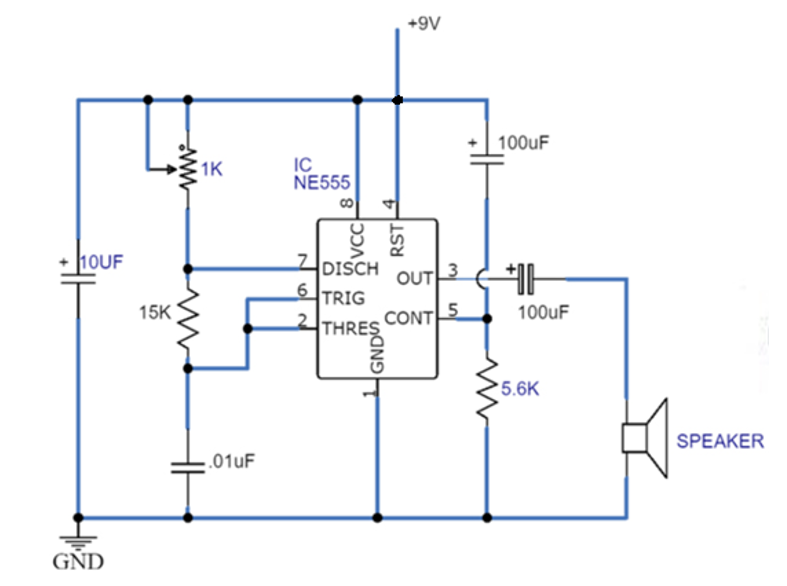
\includegraphics[width=\columnwidth]{SCHE_ORIG}
	The circuit resembles very much with the assignment 1. Some notable differences are: values of resistors and capacitors, an extra variable resistor and buzzer (speaker). A buzzer is a two-pin component that will act just like a regular resistor that produces a certain frequency of tone. It will look like this:\newline
	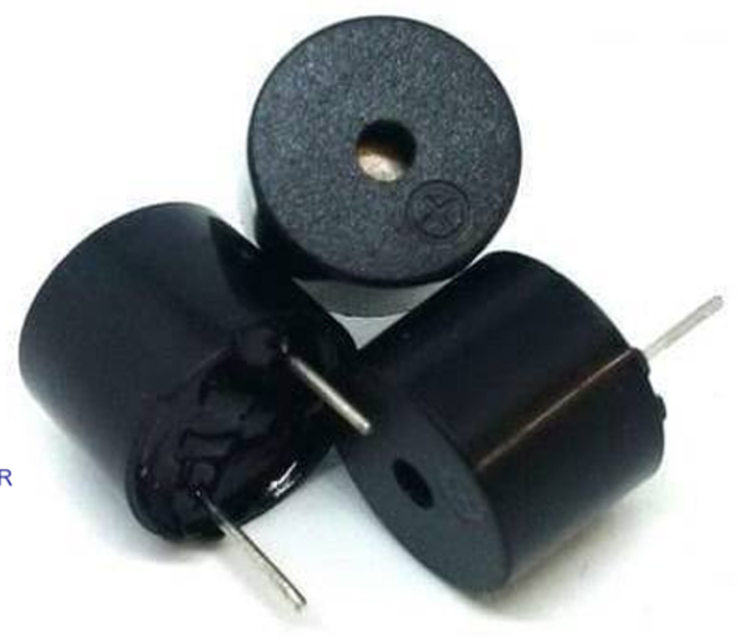
\includegraphics[width=\columnwidth]{BUZZ}
	\section{Modified Design}
	Buzzers are applicable in our real life, and one example would be the door alarm for the subway platform screen door. This is a prevalent design in east Asia, and below is a photo taken at a subway station in Singapore:\newline
	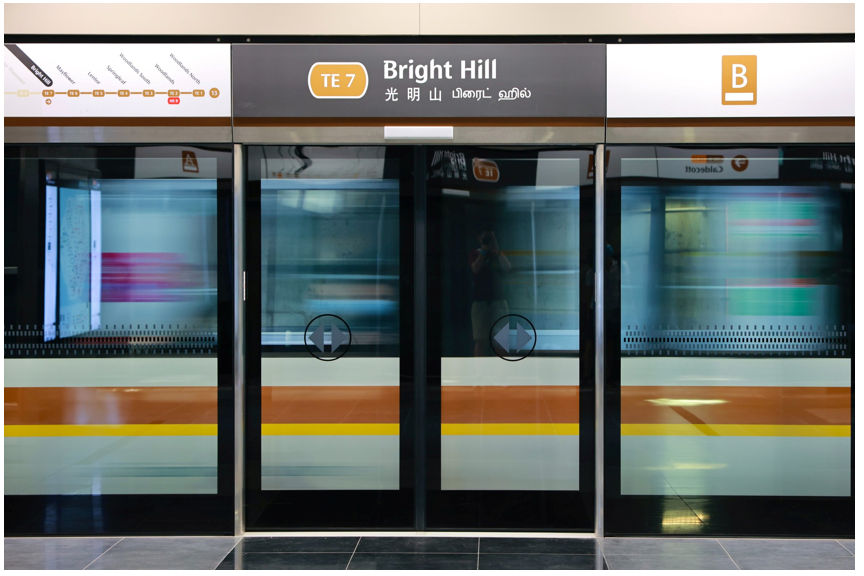
\includegraphics[width=\columnwidth]{SUBW}
	When the platform doors open, the buzzer will go off in a low frequency. On contrary, when the platform doors close, the buzzer will go off in a high frequency. Simultaneously, the LED blinks synchronously with the buzzer. \newline
	To achieve this goal, the following modifications deemed to be requisites:
	\begin{enumerate}
		\item Changing the variable resistor to a pair resistors of constant resistance, since we only need 2 frequencies.
		\item Using a switch to determine which resistors to use
	\end{enumerate}
	\subsection{Circuit Schematic}
	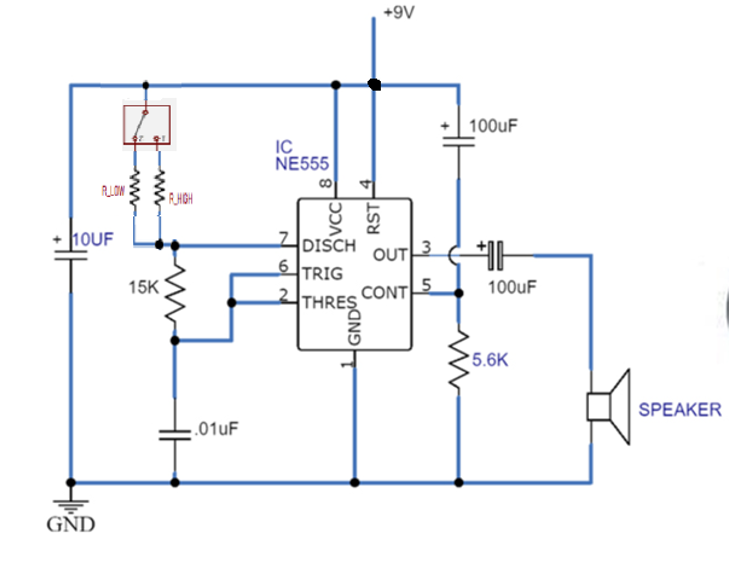
\includegraphics[width=\columnwidth]{SCHE_MODI}
	I have only drafted the circuit without exact values of the newly added resistors, as they can be arbitrary selected for desired tones.
	If everything works out well, it should have a buzzer that rings one of the two frequencies of tones. More details can be found from my presentation slides.
\end{document}